% Options for packages loaded elsewhere
\PassOptionsToPackage{unicode}{hyperref}
\PassOptionsToPackage{hyphens}{url}
%
\documentclass[
  man,floatsintext]{apa6}
\usepackage{amsmath,amssymb}
\usepackage{lmodern}
\usepackage{iftex}
\ifPDFTeX
  \usepackage[T1]{fontenc}
  \usepackage[utf8]{inputenc}
  \usepackage{textcomp} % provide euro and other symbols
\else % if luatex or xetex
  \usepackage{unicode-math}
  \defaultfontfeatures{Scale=MatchLowercase}
  \defaultfontfeatures[\rmfamily]{Ligatures=TeX,Scale=1}
\fi
% Use upquote if available, for straight quotes in verbatim environments
\IfFileExists{upquote.sty}{\usepackage{upquote}}{}
\IfFileExists{microtype.sty}{% use microtype if available
  \usepackage[]{microtype}
  \UseMicrotypeSet[protrusion]{basicmath} % disable protrusion for tt fonts
}{}
\makeatletter
\@ifundefined{KOMAClassName}{% if non-KOMA class
  \IfFileExists{parskip.sty}{%
    \usepackage{parskip}
  }{% else
    \setlength{\parindent}{0pt}
    \setlength{\parskip}{6pt plus 2pt minus 1pt}}
}{% if KOMA class
  \KOMAoptions{parskip=half}}
\makeatother
\usepackage{xcolor}
\IfFileExists{xurl.sty}{\usepackage{xurl}}{} % add URL line breaks if available
\IfFileExists{bookmark.sty}{\usepackage{bookmark}}{\usepackage{hyperref}}
\hypersetup{
  pdftitle={The Structure of Chaos: An Empirical Comparison of Fractal Physiology Complexity Indices using NeuroKit2},
  pdfauthor={Dominique Makowski1, An Shu Te1, Tam Pham1, Zen J. Lau1, \& S.H. Annabel Chen1},
  pdflang={en-EN},
  pdfkeywords={chaos, complexity, fractal, physiology, noise},
  hidelinks,
  pdfcreator={LaTeX via pandoc}}
\urlstyle{same} % disable monospaced font for URLs
\usepackage{graphicx}
\makeatletter
\def\maxwidth{\ifdim\Gin@nat@width>\linewidth\linewidth\else\Gin@nat@width\fi}
\def\maxheight{\ifdim\Gin@nat@height>\textheight\textheight\else\Gin@nat@height\fi}
\makeatother
% Scale images if necessary, so that they will not overflow the page
% margins by default, and it is still possible to overwrite the defaults
% using explicit options in \includegraphics[width, height, ...]{}
\setkeys{Gin}{width=\maxwidth,height=\maxheight,keepaspectratio}
% Set default figure placement to htbp
\makeatletter
\def\fps@figure{htbp}
\makeatother
\setlength{\emergencystretch}{3em} % prevent overfull lines
\providecommand{\tightlist}{%
  \setlength{\itemsep}{0pt}\setlength{\parskip}{0pt}}
\setcounter{secnumdepth}{-\maxdimen} % remove section numbering
% Make \paragraph and \subparagraph free-standing
\ifx\paragraph\undefined\else
  \let\oldparagraph\paragraph
  \renewcommand{\paragraph}[1]{\oldparagraph{#1}\mbox{}}
\fi
\ifx\subparagraph\undefined\else
  \let\oldsubparagraph\subparagraph
  \renewcommand{\subparagraph}[1]{\oldsubparagraph{#1}\mbox{}}
\fi
\newlength{\cslhangindent}
\setlength{\cslhangindent}{1.5em}
\newlength{\csllabelwidth}
\setlength{\csllabelwidth}{3em}
\newlength{\cslentryspacingunit} % times entry-spacing
\setlength{\cslentryspacingunit}{\parskip}
\newenvironment{CSLReferences}[2] % #1 hanging-ident, #2 entry spacing
 {% don't indent paragraphs
  \setlength{\parindent}{0pt}
  % turn on hanging indent if param 1 is 1
  \ifodd #1
  \let\oldpar\par
  \def\par{\hangindent=\cslhangindent\oldpar}
  \fi
  % set entry spacing
  \setlength{\parskip}{#2\cslentryspacingunit}
 }%
 {}
\usepackage{calc}
\newcommand{\CSLBlock}[1]{#1\hfill\break}
\newcommand{\CSLLeftMargin}[1]{\parbox[t]{\csllabelwidth}{#1}}
\newcommand{\CSLRightInline}[1]{\parbox[t]{\linewidth - \csllabelwidth}{#1}\break}
\newcommand{\CSLIndent}[1]{\hspace{\cslhangindent}#1}
\ifLuaTeX
\usepackage[bidi=basic]{babel}
\else
\usepackage[bidi=default]{babel}
\fi
\babelprovide[main,import]{english}
% get rid of language-specific shorthands (see #6817):
\let\LanguageShortHands\languageshorthands
\def\languageshorthands#1{}
% Manuscript styling
\usepackage{upgreek}
\captionsetup{font=singlespacing,justification=justified}

% Table formatting
\usepackage{longtable}
\usepackage{lscape}
% \usepackage[counterclockwise]{rotating}   % Landscape page setup for large tables
\usepackage{multirow}		% Table styling
\usepackage{tabularx}		% Control Column width
\usepackage[flushleft]{threeparttable}	% Allows for three part tables with a specified notes section
\usepackage{threeparttablex}            % Lets threeparttable work with longtable

% Create new environments so endfloat can handle them
% \newenvironment{ltable}
%   {\begin{landscape}\centering\begin{threeparttable}}
%   {\end{threeparttable}\end{landscape}}
\newenvironment{lltable}{\begin{landscape}\centering\begin{ThreePartTable}}{\end{ThreePartTable}\end{landscape}}

% Enables adjusting longtable caption width to table width
% Solution found at http://golatex.de/longtable-mit-caption-so-breit-wie-die-tabelle-t15767.html
\makeatletter
\newcommand\LastLTentrywidth{1em}
\newlength\longtablewidth
\setlength{\longtablewidth}{1in}
\newcommand{\getlongtablewidth}{\begingroup \ifcsname LT@\roman{LT@tables}\endcsname \global\longtablewidth=0pt \renewcommand{\LT@entry}[2]{\global\advance\longtablewidth by ##2\relax\gdef\LastLTentrywidth{##2}}\@nameuse{LT@\roman{LT@tables}} \fi \endgroup}

% \setlength{\parindent}{0.5in}
% \setlength{\parskip}{0pt plus 0pt minus 0pt}

% Overwrite redefinition of paragraph and subparagraph by the default LaTeX template
% See https://github.com/crsh/papaja/issues/292
\makeatletter
\renewcommand{\paragraph}{\@startsection{paragraph}{4}{\parindent}%
  {0\baselineskip \@plus 0.2ex \@minus 0.2ex}%
  {-1em}%
  {\normalfont\normalsize\bfseries\itshape\typesectitle}}

\renewcommand{\subparagraph}[1]{\@startsection{subparagraph}{5}{1em}%
  {0\baselineskip \@plus 0.2ex \@minus 0.2ex}%
  {-\z@\relax}%
  {\normalfont\normalsize\itshape\hspace{\parindent}{#1}\textit{\addperi}}{\relax}}
\makeatother

% \usepackage{etoolbox}
\makeatletter
\patchcmd{\HyOrg@maketitle}
  {\section{\normalfont\normalsize\abstractname}}
  {\section*{\normalfont\normalsize\abstractname}}
  {}{\typeout{Failed to patch abstract.}}
\patchcmd{\HyOrg@maketitle}
  {\section{\protect\normalfont{\@title}}}
  {\section*{\protect\normalfont{\@title}}}
  {}{\typeout{Failed to patch title.}}
\makeatother

\usepackage{xpatch}
\makeatletter
\xapptocmd\appendix
  {\xapptocmd\section
    {\addcontentsline{toc}{section}{\appendixname\ifoneappendix\else~\theappendix\fi\\: #1}}
    {}{\InnerPatchFailed}%
  }
{}{\PatchFailed}
\keywords{chaos, complexity, fractal, physiology, noise\newline\indent Word count: X}
\usepackage{lineno}

\linenumbers
\usepackage{csquotes}
\usepackage[titles]{tocloft}
\cftpagenumbersoff{figure}
\renewcommand{\cftfigpresnum}{\itshape\figurename\enspace}
\renewcommand{\cftfigaftersnum}{.\space}
\setlength{\cftfigindent}{0pt}
\setlength{\cftafterloftitleskip}{0pt}
\settowidth{\cftfignumwidth}{Figure 10.\qquad}
\usepackage{fvextra}
\usepackage{csquotes}
\usepackage{subfig}
\renewcommand*{\thesubfigure}{\MakeUppercase{\alph{subfigure}}}
\raggedbottom
\captionsetup[figure]{textformat=empty}
\ifLuaTeX
  \usepackage{selnolig}  % disable illegal ligatures
\fi

\title{\textbf{The Structure of Chaos: An Empirical Comparison of Fractal Physiology Complexity Indices using NeuroKit2}}
\author{Dominique Makowski\textsuperscript{1}, An Shu Te\textsuperscript{1}, Tam Pham\textsuperscript{1}, Zen J. Lau\textsuperscript{1}, \& S.H. Annabel Chen\textsuperscript{1}}
\date{}


\shorttitle{Structure of Chaos}

\authornote{

Add complete departmental affiliations for each author here. Each new line herein must be indented, like this line.

Enter author note here.

The authors made the following contributions. Dominique Makowski: Conceptualization, Data curation, Formal Analysis, Funding acquisition, Investigation, Methodology, Project administration, Resources, Software, Supervision, Validation, Visualization, Writing -- original draft; An Shu Te: Software, Project administration, Writing -- review \& editing; Tam Pham: Software, Writing -- review \& editing; Zen J. Lau: Software, Writing -- review \& editing; S.H. Annabel Chen: Project administration, Writing -- review \& editing.

Correspondence concerning this article should be addressed to Dominique Makowski, Postal address. E-mail: \href{mailto:my@email.com}{\nolinkurl{my@email.com}}

}

\affiliation{\vspace{0.5cm}\textsuperscript{1} Nanyang Technological University}

\abstract{%
One or two sentences providing a \textbf{basic introduction} to the field, comprehensible to a scientist in any discipline.

Two to three sentences of \textbf{more detailed background}, comprehensible to scientists in related disciplines.

One sentence clearly stating the \textbf{general problem} being addressed by this particular study.

One sentence summarizing the main result (with the words ``\textbf{here we show}'' or their equivalent).

Two or three sentences explaining what the \textbf{main result} reveals in direct comparison to what was thought to be the case previously, or how the main result adds to previous knowledge.

One or two sentences to put the results into a more \textbf{general context}.

Two or three sentences to provide a \textbf{broader perspective}, readily comprehensible to a scientist in any discipline.
}



\begin{document}
\maketitle

\hypertarget{introduction}{%
\section{Introduction}\label{introduction}}

Complexity is an umbrella term for concepts derived from information theory, chaos theory, and fractal mathematics, used to quantify unpredictability, entropy, and/or randomness. Using these tools to characterize signals (a subfield commonly referred to as ``fractal physiology,'' Bassingthwaighte, Liebovitch, \& West, 2013) has shown promising results in physiology in the assessment and diagnostic of the state and health of living systems Ehlers (1995).

There has been a large and accelerating increase in the number of complexity indices in the past few decades. These new procedures are usually mathematically well-defined and theoretically promising. However, few empirical evidence exist to understand their differences and similarities. Moreover, some can be very expensive in terms of computation power and thus, time, which can become an issue in some applications such as high sampling-rate techniques (e.g., M/EEG) or real-time settings (brain-computer interface). As such, having a general view depicting the relationship between the indices with information about their computation time would be useful, for instance to guide the indices selection in settings where time or computational power is limited.

One of the contributing factor of this lack of empirical comparison is the lack of free, open-source, unified, and easy to use software for computing various complexity indices. Indeed, most of them are described mathematically in journal articles, and reusable code is seldom made available, which limits their further application and validation. \emph{NeuroKit2} (Makowski et al., 2021) is a Python package for physiological signal processing that aims at providing the most comprehensive, accurate and fast pure Python implementations of complexity indices.

Leveraging this tool, the goal of this study is to empirically compare a vast number of complexity indices, inspect how they relate to one another, and extract some recommendations for indices selection, based on their added-value and computational efficiency. Using \emph{NeuroKit2}, we will compute more than a hundred complexity indices on various types of signals, with varying degrees of noise. We will then project the results on a latent space through factor analysis, and report the most interesting indices in regards to their representation of the latent dimensions.

\hypertarget{methods}{%
\subsection{Methods}\label{methods}}

\begin{figure}
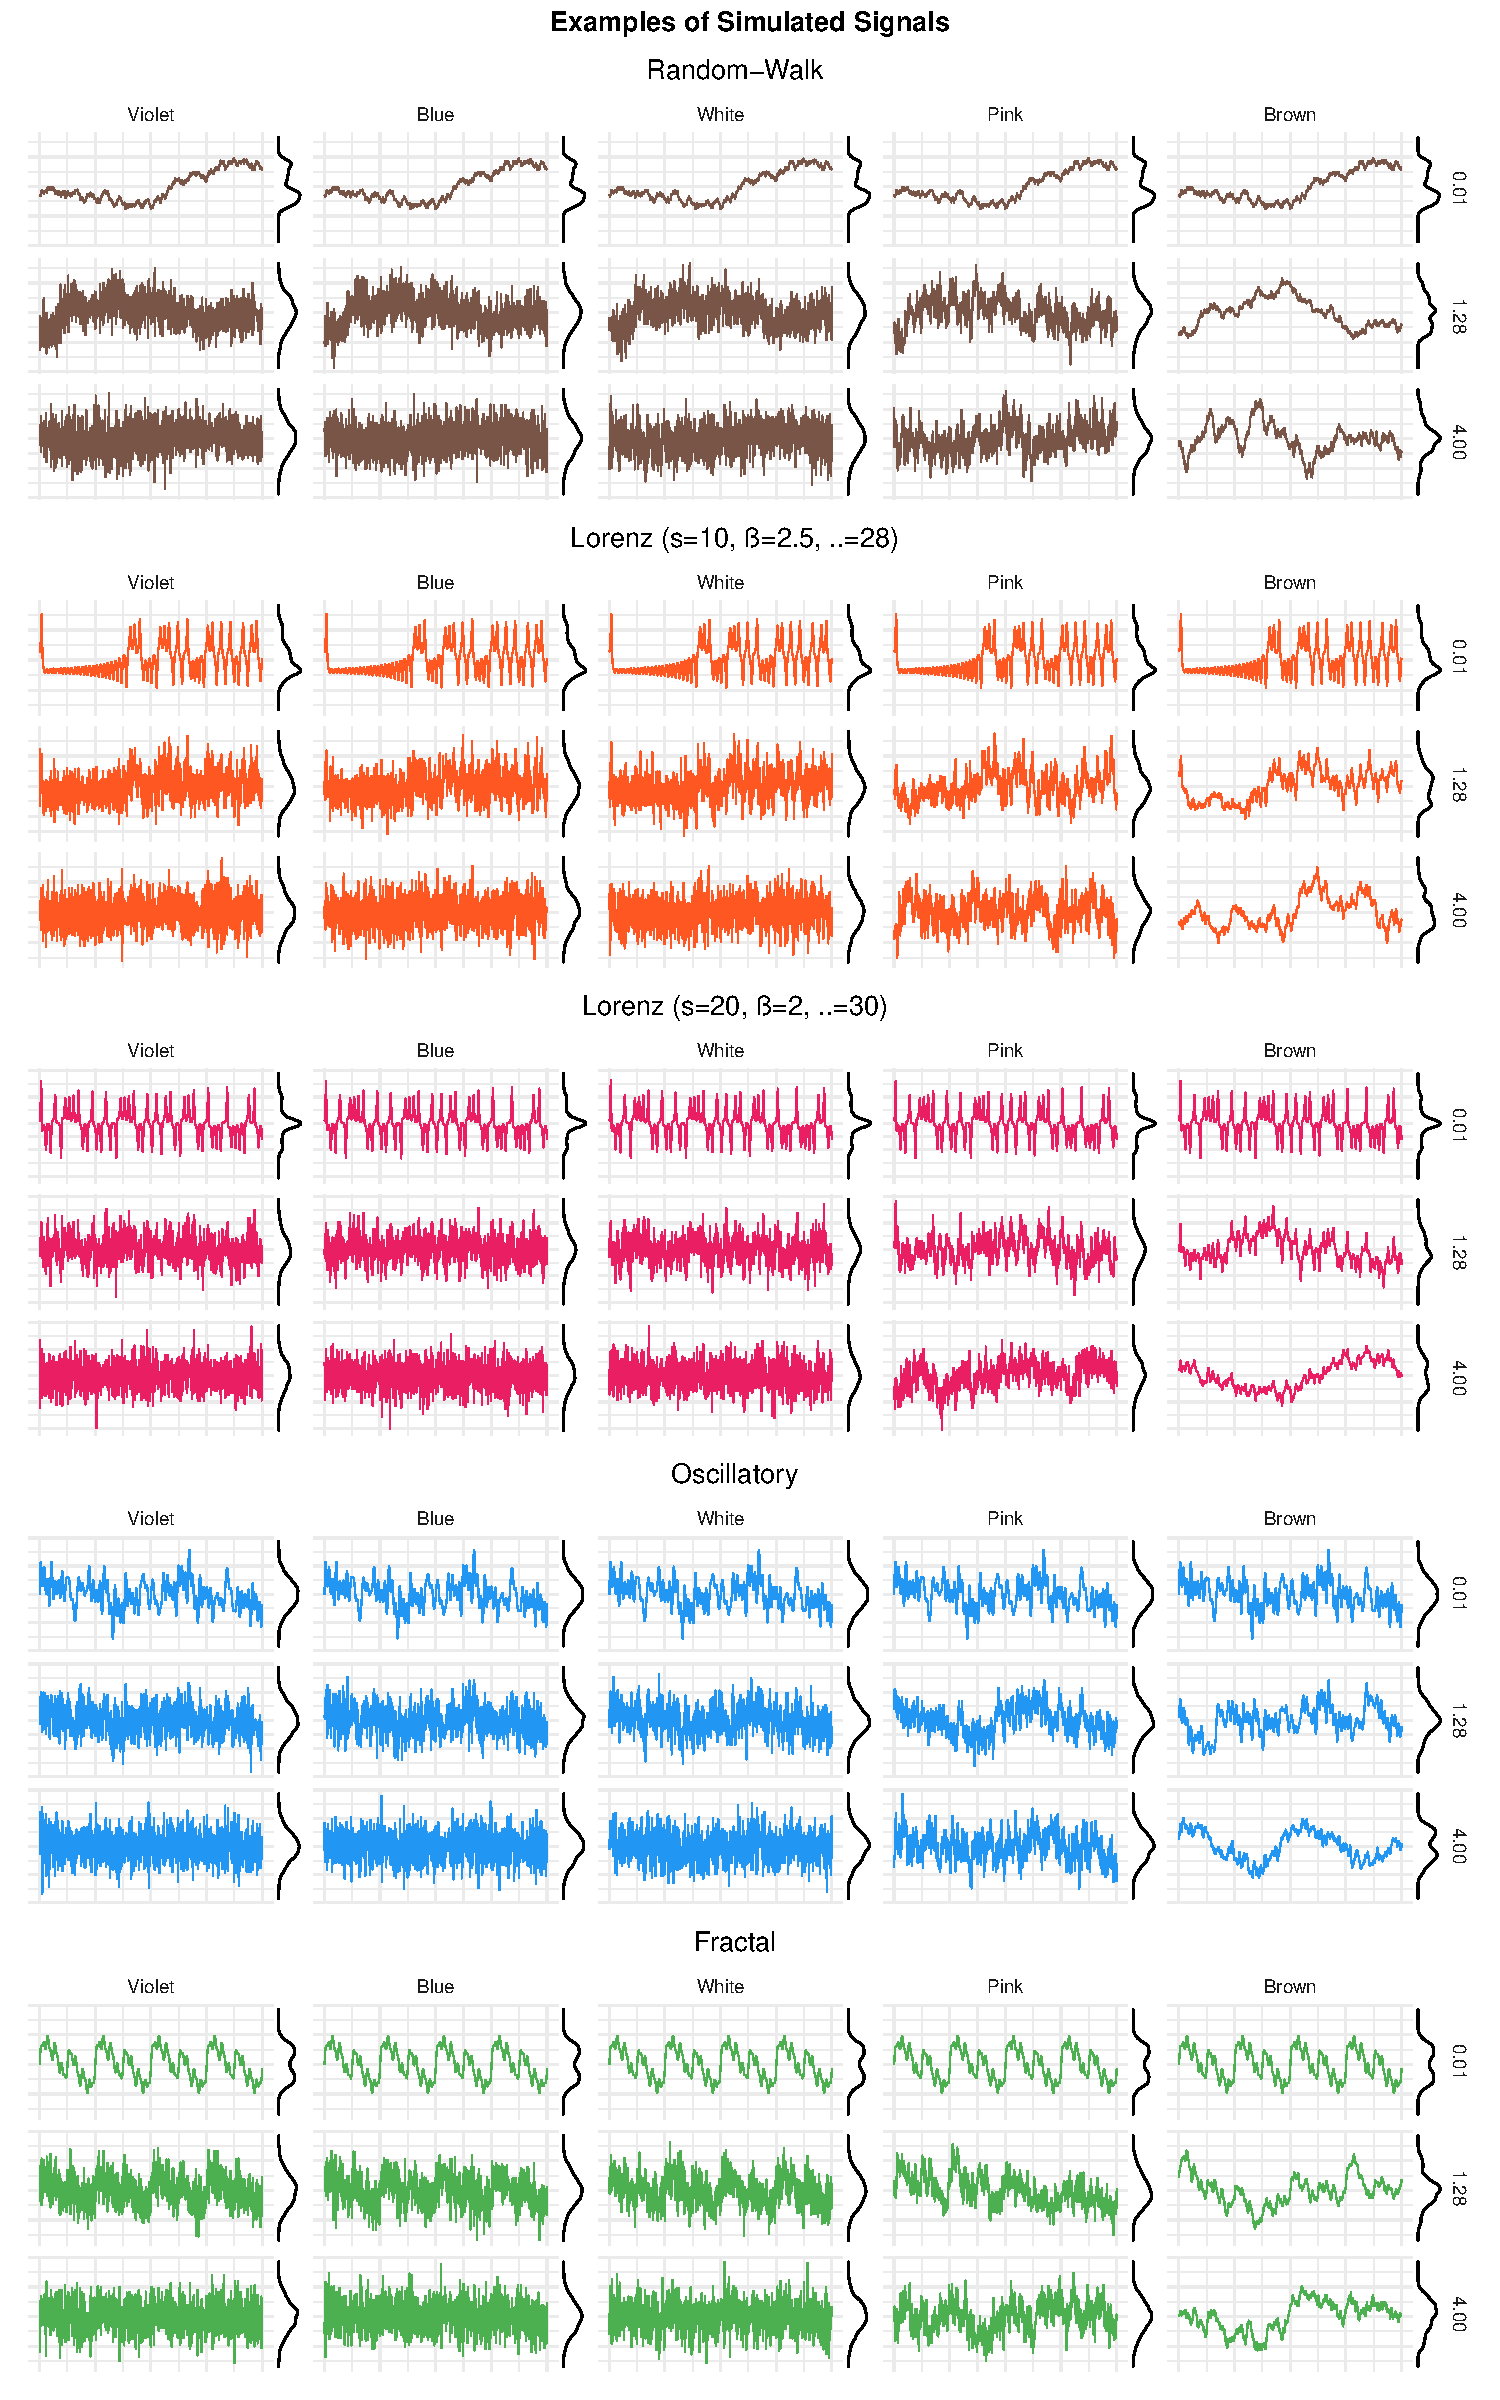
\includegraphics[width=90\%]{manuscript_files/figure-latex/fig1_signals-1} \caption{Different types of simulated signals, to which was added 5 types of noise (violet, blue, white, pink, and brown) with different intensities. For each signal type, the first row shows the signal with a minimal amount of noise, and the last with a maximal amount of noise. We can see that adding Brown noise turns the signal into a Random-walk (i.e., a Brownian motion).}(\#fig:fig1_signals)
\end{figure}

The script to generate the data can be found at \textbf{github.com/neuropsychology/NeuroKit/studies/complexity\_benchmark}

We started by generating 5 types of signals, one random-walk, two oscillatory signals made (one made of harmonic frequencies that results in a self-repeating - fractal-like - signal), and two complex signals derived from Lorenz systems (with parameters (\(\sigma = 10, \beta = 2.5, \rho = 28\)); and (\(\sigma = 20, \beta = 2, \rho = 30\)), respectively). Each of this signal was iteratively generated at \ldots{} different lengths (). The resulting vectors were standardized and each were added 5 types of \((1/f)^\beta\) noise (namely violet \(\beta=-2\), blue \(\beta=-1\), white \(\beta=0\), pink \(\beta=1\), and brown \(\beta=2\) noise). Each noise type was added at 48 different intensities (linearly ranging from 0.1 to 4). Examples of generated signals are presented in \textbf{Figure 1}.

The combination of these parameters resulted in a total of 6000 signal iterations. For each of them, we computed 128 complexity indices, and additionally basic metric such as the standard deviation (\emph{SD}), the \emph{length} of the signal and its dominant \emph{frequency}. The parameters used (such as the time-delay \(\tau\) or the embedding dimension) are documented in the data generation script. For a complete description of the various indices included, please refer to NeuroKit's documentation (\url{https://neuropsychology.github.io/NeuroKit}).

\newpage

\hypertarget{references}{%
\section{References}\label{references}}

\hypertarget{refs}{}
\begin{CSLReferences}{1}{0}
\leavevmode\vadjust pre{\hypertarget{ref-bassingthwaighte2013fractal}{}}%
Bassingthwaighte, J. B., Liebovitch, L. S., \& West, B. J. (2013). \emph{Fractal physiology}. Springer.

\leavevmode\vadjust pre{\hypertarget{ref-ehlers1995chaos}{}}%
Ehlers, C. L. (1995). Chaos and complexity: Can it help us to understand mood and behavior? \emph{Archives of General Psychiatry}, \emph{52}(11), 960--964.

\leavevmode\vadjust pre{\hypertarget{ref-lau2021brain}{}}%
Lau, Z. J., Pham, T., Annabel, S., \& Makowski, D. (2021). \emph{Brain entropy, fractal dimensions and predictability: A review of complexity measures for EEG in healthy and neuropsychiatric populations}.

\leavevmode\vadjust pre{\hypertarget{ref-Makowski2021neurokit}{}}%
Makowski, D., Pham, T., Lau, Z. J., Brammer, J. C., Lespinasse, F., Pham, H., \ldots{} Chen, S. H. A. (2021). {NeuroKit}2: A python toolbox for neurophysiological signal processing. \emph{Behavior Research Methods}, \emph{53}(4), 1689--1696. \url{https://doi.org/10.3758/s13428-020-01516-y}

\end{CSLReferences}


\clearpage
\renewcommand{\listfigurename}{Figure captions}


\end{document}
